\documentclass{standalone}
\usepackage{tikz}
\usetikzlibrary{math}

\begin{document}
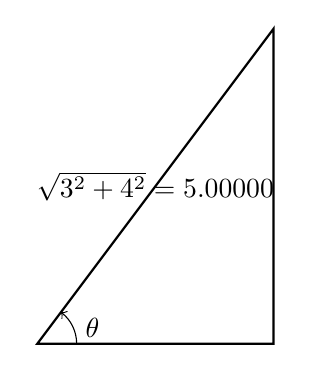
\begin{tikzpicture}
  % 使用 tikzmath 计算
  \tikzmath{
    % 定义变量
    \a = 3; \b = 4;
    % 计算斜边长度
    \c = sqrt(\a^2 + \b^2);
    % 计算角度, 不要使用 \theta (已定义)
    \angle = atan2(\b, \a);
  }

  % 绘制直角三角形
  \draw[thick] (0,0) -- (\a,0) -- (\a,\b) -- cycle;
  % 标注斜边长度
  \node at (\a/2, \b/2) {$\sqrt{\a^2 + \b^2} = \c$};
  % 标注角度
  \draw[->] (0.5,0) arc (0:\angle:0.5);
  \node at (0.7,0.2) {$\theta$};
\end{tikzpicture}
\end{document}